\begin{frame}{Toolchain}
	\begin{columns}[T]
		\begin{column}{0.55\textwidth}
			\centering
			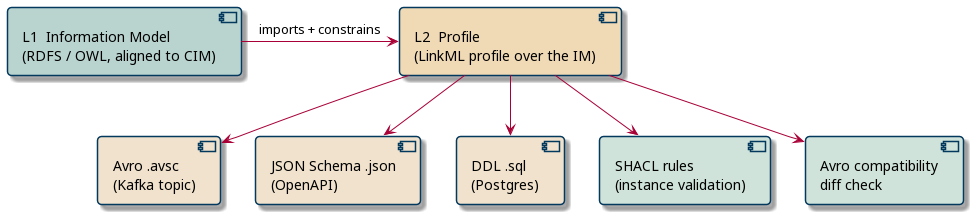
\includegraphics[width=\linewidth]{slides/exchange/consistency/figs/lifecycle.png}
		\end{column}
		\begin{column}{0.43\textwidth}
			\textbf{Consistency comes from the graph structure, not from discipline:}\\[0.4em]
			\begin{itemize}\scriptsize
				\item every artifact is \emph{downstream} of the profile
				\item a change to \texttt{PhaseCode} happens \emph{once} in the profile
				\item the validator is derived \emph{from} the same profile — one rule set
				\item review becomes: does this change the profile? what does it do to each artifact?
			\end{itemize}
		\end{column}
	\end{columns}

\end{frame}
